\section{Enzymes}
\subsection{Enzyme action}

A catalyst is a substance that increases the rate of a chemical reaction, itself remaining unchanged
at the end of the reaction.

Enzymes are protein structures that function as biological catalysts and are invovled in all 
metabolic reactions. Enzymes are composed of an active site, into which a substrate binds to 
form an enzyme-substrate complex, after which products are formed. Each enzyme only catalyses a
certain kind of reaction, as each enzyme's active site is shaped differently, only specific
substrates can fit in it. They are said to be complementarily shaped. In short, all enzymes
catalyse specific reactions, with specific substrates, as they have specifically shaped active
sites.

\subsection{Effects of temperature and pH}

The progress of enzyme catalysed reactions can be followed by measuring concentrations of reactants
and products.

With increase in temperature, enzyme activity increases as particles in the mixture have a higher
kinetic energy, increasing chances of collision of substrate with enzyme. However, beyond a certain
maximum, the enzyme activity will decrease as the protein structure of enzymes will become denatured,
and change shape. The result of this will be the active site being unable to fit their complementary
substrates. This denaturation of enzymes is permanent and cannot be reversed. 
The temperature at which the enzyme shows maximum activity is known as the optimum
temperature.

At low pH, the enzyme is also denatured, only temporarily. With increase in pH towards the
maximum, enzyme activity will increase, beyond which enzyme activity will lower for the same reason.
The pH at which enzyme activity is maximum is called the optimum pH of that enzyme.

\begin{center}
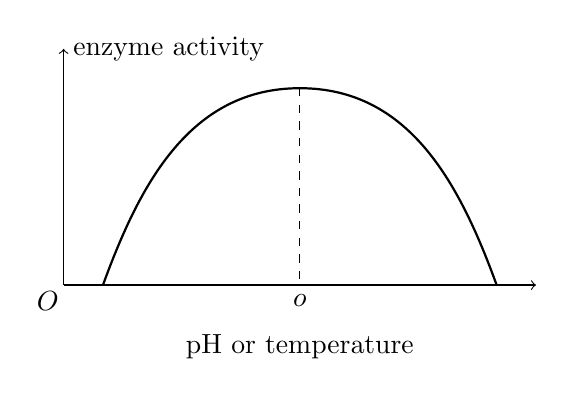
\begin{tikzpicture}

% Axes
\draw[->] (0,0) -- (6,0);
\draw (3, -0.5) node[below]{pH or temperature};
\draw[->] (0,0) -- (0,3) node[right] {enzyme activity};

% Enzyme activity curve (bell-shaped)
\draw[thick] (0.5,0) to[out=70, in=180] (3,2.5) to[out=0, in=110] (5.5,0);

% Dashes to x-axis (example points)
\draw[dashed] (3,2.5) -- (3,0) node[below] {$o$};

% Origin label
\node at (-0.2,-0.2) {$O$};

\end{tikzpicture}
\end{center}
Above is a graph where enzyme activity is plotted against pH or temperature, where $o$ is the 
optimum temperature or pH.
